\chapter{Process and methodologies}
\label{cap:process-methodologies}

\intro{In this chapter, we delve into the comprehensive exploration of the technologies employed during the internship and their broader application.}
\section{GANs}
\label{sec:gans}
\begin{figure}[H]
    \centering
    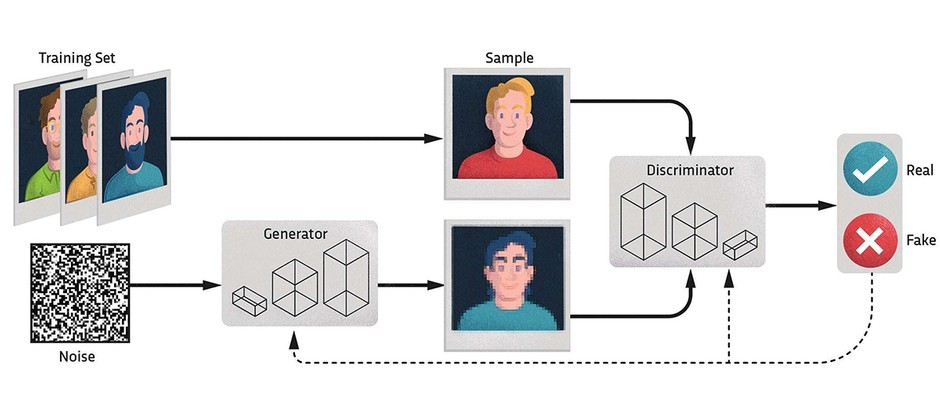
\includegraphics[width=0.75\textwidth]{images/model/gan-architecture}
    \caption{GAN architecture}\label{fig:gan-architecture}
\end{figure}

The concept of Generative Adversarial Networks (\gls{gang}) was first introduced by Ian Goodfellow and his colleagues in 2014 in their paper titled "Generative Adversarial Networks" \footcite{paper:ganpaper} published at the Neural Information Processing Systems (NIPS) conference. 
Goodfellow, along with his co-authors, proposed a novel framework that revolutionized the field of generative modeling. 
\gls{gang}s are a groundbreaking approach to generative modeling that combines elements of both supervised and unsupervised learning. 
They consist of two interconnected neural networks: a generator and a discriminator. 
The generator network learns to generate new data samples, such as images or text, by mapping random input vectors to output samples that resemble the training data. 
The discriminator network, on the other hand, aims to distinguish between real data samples from the training set and those generated by the generator. 
These two networks engage in a competitive process, where the generator strives to produce samples that the discriminator cannot differentiate from real data, while the discriminator aims to correctly classify the samples. (ref.~\ref{fig:gan-architecture}) 
Through iterative training, \gls{gang}s are able to improve the quality of the generated samples, leading to increasingly realistic and high-fidelity outputs. 
\gls{gang}s have since become a cornerstone in the field of generative modeling and have found applications in various domains, including image synthesis, text generation, and video generation. 



\section{Train process}
\label{sec:train-gan-model}
The training process of a \gls{gang} model involves a unique adversarial framework that iteratively improves the generator and discriminator networks. 
Initially, both networks are randomly initialized. During training, the generator takes random input vectors and generates synthetic data samples. 
Simultaneously, the discriminator receives both real data samples from the training set and generated samples from the generator. 
The discriminator's objective is to accurately distinguish between real and fake samples, while the generator aims to produce samples that can fool the discriminator into classifying them as real.
The training process occurs in alternating steps. In each step, the discriminator is trained by optimizing its parameters to minimize the classification error, correctly identifying real and generated samples. 
Conversely, the generator is trained by adjusting its parameters to maximize the error rate of the discriminator, essentially trying to generate samples that are indistinguishable from real data.
This adversarial game continues for multiple iterations, with the generator and discriminator networks continuously updating their weights to improve their performance. 
Through this iterative process, the generator learns to produce increasingly realistic samples, while the discriminator becomes more adept at distinguishing between real and generated data.
The training process of a \gls{gang} is complex and requires careful balancing. If the generator becomes too powerful, it may produce samples that closely resemble the training data but lack diversity. 
On the other hand, if the discriminator becomes too strong, it can easily detect generated samples, resulting in poor-quality outputs. Achieving a delicate equilibrium between the two networks is essential for training a successful \gls{gang} model.

\section{Evaluation process}
\label{sec:Evaluation-gan-model}
\subsection{The problem of evaluating GANs}
\label{subsec:problem-evaluating-gans}
In contrast to conventional deep learning models that are trained with a loss function until convergence, Generative Adversarial Networks (\gls{gang}s) operate within a zero-sum game framework involving two interconnected networks: the generator and the discriminator. 
The generator aims to deceive the discriminator by generating realistic samples, while the discriminator endeavors to accurately differentiate between genuine and fake samples. 
The training process concludes when the discriminator becomes incapable of distinguishing between real and synthetic samples, signifying that the generator has successfully captured the underlying distribution of the training data.

This unique training approach of \gls{gang}s poses a significant challenge when it comes to objective evaluation and assessment. 
Unlike traditional models that have objective functions to minimize or maximize, \gls{gang}s lack a definitive metric for gauging training progress and determining the absolute or relative performance of a \gls{gang} model solely based on loss. 
This presents several complexities in various scenarios, such as selecting a final \gls{gang} model during training, showcasing the capabilities of a \gls{gang} through generated samples, comparing different \gls{gang} models, or comparing different hyperparameters for the same \gls{gang} model.

To date, the most prevalent approach for evaluating \gls{gang}s involves a combination of qualitative and quantitative metrics that center around the quality and diversity of the generated samples.
\subsection{Manual evaluation}
\label{subsec:manual-evaluation}
Manual evaluation often serves as a means of assessing \gls{gang} models through the visual inspection of generated samples. 
This evaluation method relies on human judgment to gauge the quality of a batch of generated samples, rendering it subjective in nature. 
Although manual inspection is a straightforward approach to model evaluation, it entails several limitations. 
Firstly, subjectivity is introduced due to the evaluator's biases towards the model and the data. Secondly, expertise in the specific domain of the data is required to effectively evaluate the samples. 
Furthermore, manual evaluation is time-consuming, imposing constraints on the number of images that can be thoroughly assessed.

\emph{…evaluating the quality of generated images with human vision is expensive and cumbersome, biased […] difficult to reproduce, and does not fully reflect the capacity of models}
\footcite{paper:ganeval}.

Consequently, while manual evaluation provides an initial impression of a model's performance, it should not be solely relied upon for the final selection of a model. Fortunately, alternative and more objective evaluation methods have been proposed and embraced within the field.
\subsection{Qualitative evaluation}
\label{subsec:qualitative-evaluation}
Qualitative evaluation plays a crucial role in assessing the visual quality and performance of \gls{gang} models. 
While subjective in nature, it provides valuable insights into various aspects of the generated samples, including their fidelity, coherence, diversity, and novelty. 
Several commonly used metrics and evaluation techniques have been developed to facilitate qualitative assessment.
\begin{itemize}
    \item \textbf{Nearest neighbors}: Nearest neighbors evaluation involves comparing the generated samples with real samples from the training dataset. 
    By computing the similarity between the generated samples and their nearest neighbors in the real data space, evaluators can assess how well the \gls{gang} model captures the underlying distribution of the training data;
    \item \textbf{Rapid Scene Categorization}\footcite{paper:ganeval}: aims to evaluate the ability of GAN-generated samples to be quickly recognized and categorized by human observers. 
    Evaluators assess how well the generated samples align with the expected scene categories and their visual characteristics. This evaluation metric provides insights into the semantic coherence and overall discriminability of the generated samples;
    \item \textbf{Rating and Preference judgement}\footcite{paper:stackadvnet}\footcite{paper:stackadvnet1}\footcite{paper:stackadvnet2}\footcite{paper:stackadvnet3}:
    involve human evaluators rating or ranking the quality of generated samples based on predefined criteria. 
    This qualitative evaluation method provides subjective assessments of visual quality, realism, and aesthetic appeal. 
    By gathering ratings or preference judgments from multiple evaluators, a collective assessment of the generated samples can be obtained;
    \item \textbf{Mode Drop and Collapse}\footcite{paper:dropandcollapse}\footcite{paper:dropandcollapse2}: Mode drop and collapse refer to situations where the \gls{gang} model fails to generate samples representing all the diverse modes or aspects of the training data distribution. 
    Evaluators visually inspect the generated samples to identify any mode drop, where certain modes or patterns are missing, or mode collapse, where the generated samples lack diversity and exhibit repetitive patterns. 
    Assessing mode drop and collapse is crucial for evaluating the ability of \gls{gang} models to capture the full range of variations in the training data;
    \item \textbf{Network Internals}\footcite{paper:netint}\footcite{paper:netint1}\footcite{paper:netint2}\footcite{paper:netint3}\footcite{paper:netint4}\footcite{paper:netint5}: 
    Analyzing the internal representations and activations of the \gls{gang} model's neural network can provide insights into the learning process and the generated samples' quality. 
    Evaluators examine network internals, such as feature maps and intermediate layers, to gain a better understanding of how the GAN model generates and captures visual patterns;
\end{itemize}
The most used qualitative measure is a sort of manual inspection of images, called \emph{Rating and Preference judgement}.\\\\
\emph{\dots These types of experiments ask subjects to rate models in terms of the fidelity of their generated images\dots}\footcite{paper:ganeval}.\\\\
Usually images are shown in pairs (one real and one fake), and the subjects are asked to choose the best image.
A score or rating is then assigned to the model based on the number of times it is chosen as the best image.
For lowering the variance of the results, the images are shown to multiple human judges and the results are averaged.
This process is labor intensive, but with the help of crowd-sourcing platforms like Amazon Mechanical Turk, 
it can be done at scale (Reducing the cost also).\\
Another downside of this method is that the human judges performance can improve with experience, especially if they are given feedback on their performance.\\\\
\emph{\dots By learning from such feedback, annotators are better able to point out the flaws in generated images, giving a more pessimistic quality assessment\dots}\footcite{paper:ganeval}.\\\\
\subsection{Quantitative evaluation}
\label{subsec:quantitative-evaluation}
In addition to qualitative evaluation, quantitative assessment provides a systematic and objective analysis of \gls{gang} models' performance. 
These evaluation metrics aim to measure various aspects of the generated samples, including their diversity, fidelity, and similarity to the real data distribution. 
By quantitatively evaluating \gls{gang} models, researchers can compare different models, assess the impact of hyperparameters, and track progress during training.
Some of the most common quantitative measures are: Average log-likelihood, Coverage Metric, Inception Score, Modified Inception Score, Mode Score, AM Score, Fréchet Inception Distance, 
Maximum Mean Discrepancy, The Wasserstein Distance, Birthday Paradox Test, Classifier Two-Sample Tests, Classification Performance, Boundary Distortion, 
Number of Statistically-Different Bins, Image Retrieval Performance, Generative Adversarial Metric, Tournament Win Rate, Normalized Relative Discriminative Score, Adversarial Accuracy and Adversarial Divergence, 
Geometric Score, Reconstruction Score, Image Quality measures, Low-level Image Statistics, Precision, Recall and F1 Score.
%Quantitative measures are based on the use of metrics to evaluate the quality of the generated samples.
%All this methods use a numerical score to evaluate the quality.
%Some of the most common quantitative measures are: Average log-likelihood, Coverage Metric, Inception Score, Modified Inception Score, Mode Score, AM Score, Fréchet Inception Distance, Maximum Mean Discrepancy, The Wasserstein Distance, Birthday Paradox Test, Classifier Two-Sample Tests, Classification Performance, Boundary Distortion, Number of Statistically-Different Bins, Image Retrieval Performance, Generative Adversarial Metric, Tournament Win Rate, Normalized Relative Discriminative Score, Adversarial Accuracy and Adversarial Divergence, Geometric Score, Reconstruction Score, Image Quality measures, Low-level Image Statistics, Precision, Recall and F1 Score.\\
%%\begin{itemize}
%%    \item Average log-likelihood;
%%    \item Coverage Metric;
%%    \item Inception Score;
%%    \item Modified Inception Score;
%%    \item Mode Score;
%%    \item AM Score;
%%    \item Frechet Inception Distance;
%%    \item Maximum Mean Discrepancy;
%%    \item The Wasserstein Distance;
%%    \item Birthday Paradox Test;
%%    \item Classifier Two-Sample Tests;
%%    \item Classification Performance
%%    \item Boundary Distortion 
%%    \item Number of Statistically-Different Bins
%%    \item Image Retrieval Performance
%%    \item Generative Adversarial Metric
%%    \item Tournament Win Rate
%%    \item Normalized Relative Discriminative Score
%%    \item Adversarial Accuracy and Adversarial Divergence
%%    \item Geometric Score
%%    \item Reconstruction Score
%%    \item Image Quality measures
%%    \item Low-level Image Statistics
%%    \item Precision, Recall and F1 Score
%%\end{itemize}

The most used quantitative measures are \textbf{\emph{Inception Score}} and \textbf{\emph{Fréchet Inception Distance}}.
\subsubsection{Inception Score}
\label{subsubsec:inception-score}
The Inception Score (\gls{ISG}\glsfirstoccur) is a widely used quantitative metric for evaluating the quality and diversity of generated samples in \gls{gang} models.
It was proposed in 2016 by Tim Salimans et al. in \emph{"Improved Techniques for Training GANs"}\footcite{paper:salimans2016improved}, provides a measure of both sample quality and class diversity. 
The \gls{ISG} is computed by first obtaining the predicted class probabilities for each generated sample using an Inception-v3 pre-trained classifier. 
Then, the average of these probabilities is calculated to assess the quality of the generated samples. 
Additionally, the entropy of the predicted class probabilities is computed to measure the diversity of the samples. 
The formula for calculating the Inception Score is as follows:
\begin{equation}
    \label{eq:inception-score}
    \text{IS} = \exp \left( \mathbb{E}_{\mathbf{x} \sim p_{\text{data}}} \left[ \text{KL} \left( p(y|\mathbf{x}) || p(y) \right) \right] \right)
\end{equation}
The KL divergence is a measure of how one probability distribution is different from a second, reference probability distribution.
The KL divergence is defined as:
\begin{equation}
    \label{eq:kl-divergence}
    \text{KL}(P || Q) = \sum_{i} P(i) \log \left(\frac{P(i)}{Q(i)}\right)
\end{equation}
The Inception Score is a good measure of the quality of generated images, but it has some limitations.
It is sensitive to dataset and classifier choice, lacks consideration of spatial coherence, may not detect mode collapse effectively, offers limited interpretability, and emphasizes high-quality samples. 
Complementary metrics and qualitative assessments are essential for a comprehensive evaluation of \gls{gang} models.
\subsubsection{Frechet Inception Distance}
\label{subsubsec:frechet-inception-distance}
The Fréchet Inception Distance (\gls{fidg}\glsfirstoccur) score is a widely used metric for evaluating the quality of generated images in the field of generative adversarial networks (GANs) introduced by Martin Heusel et al. \footcite{paper:heusel2017gans}. 
\\\\
\emph{"\gls{fidg} performs well in terms of discriminability, robustness and computational efficiency [...] It has been shown that \gls{fidg} is consistent with human judgments and is more robust to noise than \gls{ISG}".}\footcite{paper:ganeval}\\\\
It measures the similarity between the distribution of real images and the distribution of generated images by comparing their feature representations extracted from a pre-trained Inception-v3 network\footcite{paper:inceptionv3}. 
A lower \gls{fidg} score indicates better similarity between the two distributions, suggesting higher-quality generated images that resemble the real data more closely. 
The \gls{fidg} score takes into account both the quality and diversity of generated images, making it a valuable metric for assessing the performance of \gls{gang} models. 
It provides a quantitative measure that complements visual inspection and subjective evaluation, enabling researchers to objectively compare and analyze different \gls{gang} architectures and training strategies.
The \gls{fidg} score is defined as:
\begin{equation}
    \label{eq:fid-score}
    \text{FID}(p, q) = \|\mu_p - \mu_q\|^2 + \text{Tr}(\Sigma_p + \Sigma_q - 2(\Sigma_p\Sigma_q)^{1/2})
\end{equation}
Where:
\begin{itemize}
    \item $\mu_p$ and $\mu_q$ are the mean vectors of the real and generated images respectively.
    \item $\Sigma_p$ and $\Sigma_q$ are the covariance matrices of the real and generated images respectively.
    \item \text{Tr} is the trace operator.
    \item $\|\cdot\|$ is the Euclidean norm.
\end{itemize}
As the \gls{ISG} score, the \gls{fidg} score has some limitations based on the use of the Inception-v3 network.
\subsubsection{Suggested GAN evaluation procedure}
\label{subsubsec:suggested-gan-evaluation-procedure}
The evaluation of Generative Adversarial Networks (\gls{gang}s) presents challenges, necessitating a comprehensive approach that combines qualitative and quantitative measures. 
Initially, a manual inspection of the generated images is recommended to assess the quality of the generator model. Subsequently, quantitative measures such as the Inception Score and the Frechet Inception Distance can be employed to evaluate the quality and diversity of the generated images. 
It is important to note that there is no universally superior measure for \gls{gang} evaluation, as the selection of evaluation measures depends on the specific task and dataset at hand.\\\\
\emph{
    As of yet, there is no consensus regarding the best score. Different scores assess various aspects of the image generation process, and it is unlikely that a single score can cover all aspects. Nevertheless, some measures seem more plausible than others (e.g. \gls{fidg} score)
}\footcite{paper:ganeval}